%label:"art:ASideLandauGinzburgModel"
%type:"article"
%name:"$A$-side Landau-Ginzburg model"
%caption:""
%parent:"art_HMSForFanos2"


On this side of the mirror, $Y$ will be a K\"ahler manifold, along with a holomorphic function $W: Y \to \CC$ which is:
\begin{itemize}
    \item Proper (or controlled at $\infty$ in the fiber directions)
    \item A fibration near $\infty$ or has smooth fibers.
\end{itemize}
The objects of the Fukaya-Seidel category $\FS(Y, W)$ are Lagrangian submanifolds $L \subset Y$ such that $W|_L$ is a fibration over $\RR_+$ outside of a compact set. 

%label:"fig:LagrangiansInTheFukayaSeidelCategory"
%type:"figure"
%name:"Lagrangians in the Fukaya Seidel Category"
%caption:"A Lagrangian submanifold in a Fukaya-Seidel category needs to have prescribed behavior going off to infinity."
%parent:"art_ASideLandauGinzburgModel"


    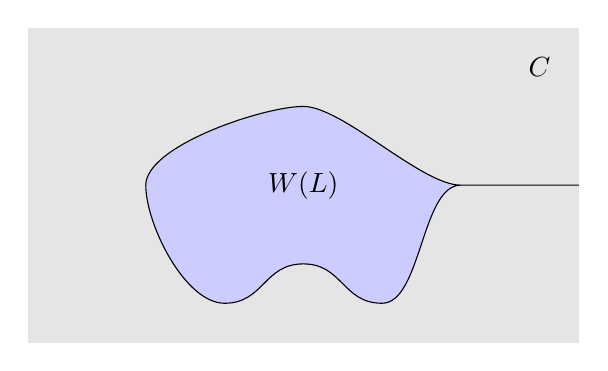
\begin{tikzpicture}

        \fill[gray!20] (-3,2.5) rectangle (4,-1.5);
        \draw[fill=blue!20] (2.5,0.5) .. controls (2,0.5) and (1,1.5) .. (0.5,1.5) .. controls (0,1.5) and (-1.5,1) .. (-1.5,0.5) .. controls (-1.5,0) and (-1,-1) .. (-0.5,-1) .. controls (0,-1) and (0,-0.5) .. (0.5,-0.5) .. controls (1,-0.5) and (1,-1) .. (1.5,-1) .. controls (2,-1) and (2,0.5) .. (2.5,0.5) .. controls (4,0.5) and (3,0.5) .. (4,0.5);
        \node at (0.5,0.5) {$W(L)$ };
        \node at (3.5,2) {$\mathbb{C}$};
    \end{tikzpicture}



To take the Lagrangian intersection Floer cohomology between two such Lagrangians, we need to perturb the Lagrangians at infinity; the perturbation we take will rotate one Lagrangian at infinity. 
As a vector space, $\hom(L, K) = \CC(\langle L \cap \phi(K)\rangle)$.
%label:"fig:PushoffInFukayaSeidelCategory"
%type:"figure"
%name:"pushoff in Fukaya-Seidel category"
%caption:"To obtain transversality, the Lagrangian submanifolds in the Fukaya-Seidel category are pushed off one another with respect to the projection $W: Y \to \CC$."
%parent:"art_ASideLandauGinzburgModel"


    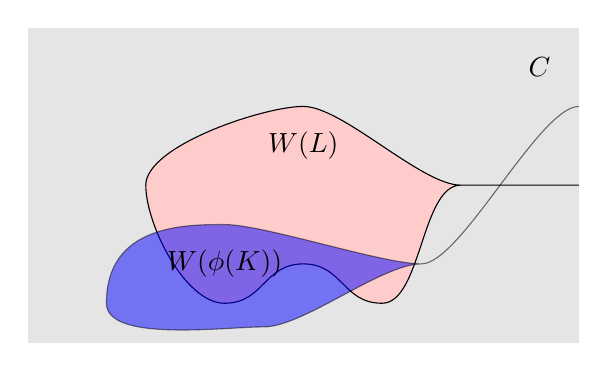
\begin{tikzpicture}

        \fill[gray!20] (-3,2.5) rectangle (4,-1.5);
        \draw[fill=red!20] (2.5,0.5) .. controls (2,0.5) and (1,1.5) .. (0.5,1.5) .. controls (0,1.5) and (-1.5,1) .. (-1.5,0.5) .. controls (-1.5,0) and (-1,-1) .. (-0.5,-1) .. controls (0,-1) and (0,-0.5) .. (0.5,-0.5) .. controls (1,-0.5) and (1,-1) .. (1.5,-1) .. controls (2,-1) and (2,0.5) .. (2.5,0.5) .. controls (4,0.5) and (3,0.5) .. (4,0.5);
        \node at (0.5,1) {$W(L)$ };
        \node at (3.5,2) {$\mathbb{C}$};
        \draw[fill=blue, opacity=.5] (-0.5,0) .. controls (-1,0) and (-2,0) .. (-2,-1) .. controls (-2,-1.5) and (-0.5,-1.3) .. (0,-1.3) .. controls (0.5,-1.3) and (1.5,-0.5) .. (2,-0.5) .. controls (2.5,-0.5) and (3.5,1.5) .. (4,1.5) .. controls (3.5,1.5) and (2.5,-0.5) .. (2,-0.5) .. controls (1.5,-0.5) and (0,0) .. (-0.5,0);
        \node at (-0.5,-0.5) {$W(\phi(K))$};
    \end{tikzpicture}


The differential and product structure on hom-spaces is given by counts of pseudo-holomorphic disks. 

%label:"art:ComparisonToBSide"
%type:"article"
%name:"Comparison to $B$-side"
%caption:""
%parent:"art_ASideLandauGinzburgModel"


Let $\CritVal(W) \subset \CC$ be the subset of critical values of $W$. For each $c \in \CritVal(W)$, we have a ``smaller'' Landau-Ginzburg model $Y_c$ by trivially extending $W^{-1}(B(c, \epsilon)) \to B(c, \epsilon)$ to a fibration over $\CC$. 
%label:"fig:SmallNeighborhoodFsCategory"
%type:"figure"
%name:"small neighborhood FS category"
%caption:"A small neighborhood in the base of a symplectic LG model can be used to build another LG model."
%parent:"art_ComparisonToBSide"


    \begin{tikzpicture}

        \draw (-3,2.5) rectangle (4,-1.5);
        
        
        \node at (3.5,2) {$\mathbb{C}$};
        
        
        \node at (-1,0) {$\times$};
        \node at (1.5,0.5) {$\times$};
        \node at (-1,1.5) {$\times$};
        \draw[dotted]  (-1,1.5) ellipse (0.5 and 0.5);
        \node at (0,1.5) {$B(c, \epsilon)$};
    \end{tikzpicture}


Define $\FS_c = \FS(Y_c, W)$. 
%label:"def:VanishingPath"
%type:"definition"
%name:"vanishing path"
%caption:""
%parent:"art_ComparisonToBSide"


Let $c \in \CritVal(W)$ be a critical point. A \emph{vanishing path} for $c$ is a path $\gamma: [0, \infty) \to \CC$ such that 
\begin{itemize}
\item $\gamma(0) = c$ 
\item $\gamma$ avoids all other critical values 
\item $\gamma(t) = t$ for $t \gg 0$. 
\end{itemize}


A vanishing path determines an embedding $\FS_c \to \FS(Y, W)$ by extending Lagrangian submanifolds over the vanishing path using symplectic parallel transport. 
%label:"fig:ExtendingByVanishingPath"
%type:"figure"
%name:"extending by vanishing path"
%caption:"A vanishing path determines a method for extending Lagrangians belonging to the Fukaya-Seidel category near a critical value to the Fukaya-Seidel category of $(Y, W)$."
%parent:"art_ComparisonToBSide"


    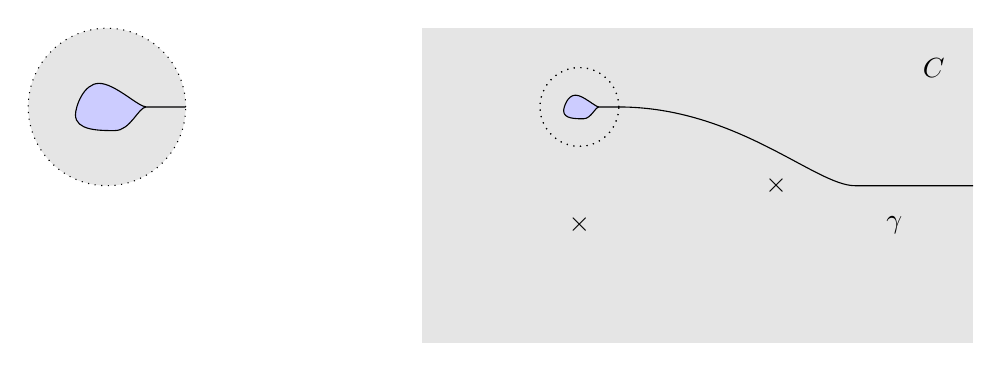
\begin{tikzpicture}

        \fill[gray!20] (-3,2.5) rectangle (4,-1.5);
        
        
        \node at (3.5,2) {$\mathbb{C}$};
        
        
        \node at (-1,0) {$\times$};
        \node at (1.5,0.5) {$\times$};
        \node at (-1,1.5) {$\times$};
        \draw[dotted]  (-1,1.5) ellipse (0.5 and 0.5);
        
        \begin{scope}[]
        \draw[dotted, fill=gray!20] (-7,1.5) ellipse (1 and 1);
        \draw[fill=blue!20] (-6,1.5) .. controls (-6.1,1.5) and (-6.4,1.5) .. (-6.5,1.5) .. controls (-6.6,1.5) and (-6.9,1.8) .. (-7.1,1.8) .. controls (-7.3,1.8) and (-7.4,1.5) .. (-7.4,1.4) .. controls (-7.4,1.2) and (-7.1,1.2) .. (-6.9,1.2) .. controls (-6.7,1.2) and (-6.6,1.5) .. (-6.5,1.5);
        
        \end{scope}
        
        
        \begin{scope}[scale=0.5, shift={(5,1.5)}]
        \draw[dotted] (-7,1.5) ellipse (1 and 1);
        \draw[fill=blue!20] (-6,1.5) .. controls (-6.1,1.5) and (-6.4,1.5) .. (-6.5,1.5) .. controls (-6.6,1.5) and (-6.9,1.8) .. (-7.1,1.8) .. controls (-7.3,1.8) and (-7.4,1.5) .. (-7.4,1.4) .. controls (-7.4,1.2) and (-7.1,1.2) .. (-6.9,1.2) .. controls (-6.7,1.2) and (-6.6,1.5) .. (-6.5,1.5);
        
        \end{scope}
        
        
        \draw (-0.5,1.5) .. controls (1,1.5) and (2,0.5) .. (2.5,0.5) .. controls (3,0.5) and (3.5,0.5) .. (4,0.5);
        \node at (3,0) {$\gamma$};
    \end{tikzpicture}


If we choose ``disjoint'' vanishing paths, we get a semi-orthogonal decomposition:
\[\FS(Y, W) = \langle \FS_1, \ldots, \FS_n\rangle \]

%label:"exm:MirrorSymmetryForTheProjectivePlane"
%type:"example"
%name:"mirror symmetry for the projective plane"
%caption:""
%parent:"art_ComparisonToBSide"


\label{exm:HMSforP2}
Consider the symplectic Landau-Ginzburg model whose critical points are arranged as follows:
%label:"fig:VanishingPathsForP2"
%type:"figure"
%name:"vanishing paths for P2"
%caption:"A set of vanishing paths for the Lefschetz fibration $W(z_1, z_2) = z_1 + z_2 + (z_1z_2)^{-1}$"
%parent:"exm_MirrorSymmetryForP2"


    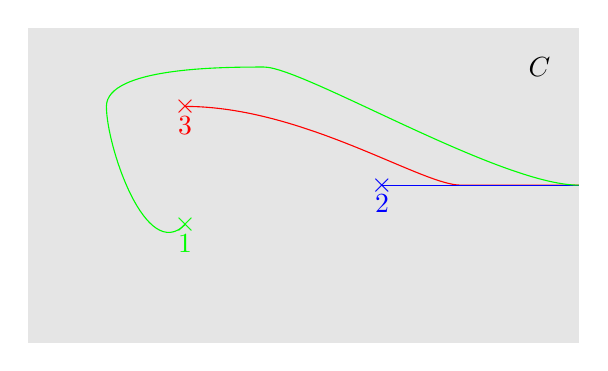
\begin{tikzpicture}

        \fill[gray!20] (-3,2.5) rectangle (4,-1.5);
        
        \node at (3.5,2) {$\mathbb{C}$};
        
        \node[green] at (-1,0) {$\times$};
        \node[blue] at (1.5,0.5) {$\times$};
        \node[red] at (-1,1.5) {$\times$};
        
        \node[below,green] at (-1,0) {$1$};
        \node[below,blue] at (1.5,0.5) {$2$};
        \node[below,red] at (-1,1.5) {$3$};
        \draw[red] (-1,1.5) .. controls (0.5,1.5) and (2,0.5) .. (2.5,0.5) .. controls (3,0.5) and (3.5,0.5) .. (4,0.5);
        \draw[blue] (1.5,0.5) -- (4,0.5);
        \draw[green] (-1,0) .. controls (-1.5,-0.5) and (-2,1) .. (-2,1.5) .. controls (-2,2) and (-0.5,2) .. (0,2) .. controls (0.5,2) and (3,0.5) .. (4,0.5);
    \end{tikzpicture}


 We obtain a semi-orthogonal decomposition $\FS(Y, W) = \langle \FS_1, \FS_2, \FS_3 \rangle$.





%label:"art:ExceptionalCollections"
%type:"article"
%name:"Exceptional collections"
%caption:""
%parent:"art_ASideLandauGinzburgModel"


Suppose additionally that $W^{-1}(c)$ has an $A_1$ singularity (a node) then 
\[\FS_c = D\Coh(\text{pt}) = D\Vect\]
and the generating object is called the \emph{vanishing thimble} associated with the point. So if all critical points of $W$ are more (i.e., $W$ is a Lefschetz fibration), then $\FS(Y, W)$ admits a full exceptional collection. 

If $W$ has isolated singularities, they can be ``Morsified'' by a small perturbation (in the symplectic category). From this, we obtain the following principle:
if $(Y, W)$ is a symplectic Landau-Ginzburg model and $W$ has isolated singularities, then $\FS(Y, W)$ admits a full exceptional collection. 
This tells us that many examples arising from mirror symmetry will \emph{not} have isolated singularities, as their mirror spaces will not have full exceptional collections! However, we still have the following expectations. When $X$ is Fano, and $(Y, W)$ is its mirror, then we expect $W$ will have some isolated singularities, and an additional critical value $c_{\text{Ku}}$ with non-isolated singularities with 
\[\text{Ku}(X) = \FS_{c_{\text{Ku}}}.\]



